% $Id: AllegProposal.tex,v 1.8 2000/07/05 21:02:12 culver Exp $
% AllegProposal.tex
% by A. Thall
% 13. Feb 2003
%
% Small edits and a few additions made by R. Roos
% 21 Jan 2007
% Most particularly, the "box" around the thesis statement has been removed,
% section titles have been modified. The section named "Prior work II" has
% been commented out. The \topmargin has been changed to -.5in and the
% change to \parindent has been commented out.
% The filename "nausicaa.eps" has been changed to simply "nausicaa" so that
% pdflatex can be used on the file (and a file named "nausicaa.pdf" has
% been created using the "epstopdf" command).
% Several subsections have been added to illustrate subsection usage.
% The word "comp" has been replaced by "project" or "thesis" throughout.
% Other small changes have been made.
%
% This document provides a sample Senior Project Proposal template for use
% by students in Allegheny's CS and Applied Computing programs.

\NeedsTeXFormat{LaTeX2e}
\documentclass[12pt]{article}

%The following is used by WinEdt to set up cross-referencing to the BibTeX files
%It is NOT commented out---the comment lets it be simply ignored by non-WinEdt LaTeX compilers

%GATHER{mybibtexDB.bib}

\usepackage{setspace}
\usepackage{amsmath}
\usepackage{amssymb}
\usepackage{epsfig}
\usepackage{fancybox}
\usepackage{listings}
\usepackage{algo}
\usepackage{url}
\usepackage{hyperref}

% for watermakr
\usepackage{graphicx}
%\usepackage{tikz}
%\usepackage{eso-pic}

%\newcommand\BackgroundPicA{\put(-50,50){{
%\begin{tikzpicture}\node[opacity=0.15]{
%\includegraphics[scale=5.0]{test.png}};
%\end{tikzpicture}%
%}}}

%\makeatletter
%\AddToShipoutPicture{\BackgroundPicA}
%\makeatother

\setlength{\textheight}{9in}
\setlength{\textwidth}{6in}
\setlength{\oddsidemargin}{.25in}
\setlength{\topmargin}{-.5in}  % changed from -.25 by RSR on 1/21/07
%\parindent .5in    % commented out by RSR 1/21/07

%put words in the hyphenation statement if you want to enforce
%how LaTeX should break them (or not) at the end of a line.
%\hyphenation{repre-sen-tations problems exact linear}
\hyphenation{itself}

%%%%%
%% Commented out -- RSR, 1/21/07
%%%%%
% The following provides a box to surround the thesis statement
%\newenvironment{Thesis}%
%{\begin{Sbox}\begin{minipage}{.95\linewidth}}%
%{\end{minipage}\end{Sbox}\begin{center}\fbox{\TheSbox}\end{center}}

\title{Sol-MakerMKII: Arduino Uno Based Solenoid Controller}
\author{Steven A. Bj\o rnson}

\begin{document}

% You can specify a language and other options for
% the code-formatting "listings" package
\lstset{language=C++,basicstyle=\small,
        stringstyle=\ttfamily,showstringspaces=false}

\singlespace
\maketitle

\doublespace
% This sets section-numbering to only include Section and Subsection numbers
\setcounter{secnumdepth}{2}

\section{Outline:}\label{ch:overview}

The Sol-Maker MKII is a shield designed for the Arduino Uno. This shield allows for individual control of up to twelve solenoids (push, pull, or rotary) utilizing an external power supply; 12 or 24 volts depending on the power requirements of the solenoids. Control of each solenoid is made possible by communication with each of the 12 output pins on the Arduino Uno�1 pin per solenoid. The current code compiled on the Ardiuino allows the user to send messages on/off messages from a computer to the Arduino via the USB port.

\section{Circuit:}
The design of the circuit is quite simple. Each of the 12 digital outputs of the Arduino Uno (outputs 2 to 13) are connected to identical modules. Each module contains a resistor, a TIP120 transistor, and a diode. These modules allow the shared voltage (12 or 24 volt external power supply) to be controlled by the digital output of the Arduino for each solenoid.

	In each module the TIP120 acts as a gate which is opened and closed by the 5 volt output from the digital output pins of the Arduino. The resistor is necessary since the TIP120  provides very low impedance and so without it the Arduino could be damaged. 

		A diode is run in parallel with each solenoid. This is necessary because solenoids are inductors and after a solenoid is cycled (charged and released) the plunger returns to the starting point (by way of mechanical potential energy; a spring or gravity will return the plunger to home). This returning plunger pushes current the opposite direction in the circuit and thus without the diode this reversed current could potentially damage the transistor.

	The second section of each module contains a resistor and an light emitting diode (LED). This section is connected in parallel to each of the digital output pins which control the solenoids. When a solenoid is activated, a corresponding LED is activated. The LEDs are powered by the 5V provided by the digital outputs and do not utilize the external power supply. 

		A resistor in series with the LED provides the same function as the TIP120's resistor. 

		The purpose of the LED is to provide visual feedback and, since it will continue to operate when the external power supply is not on and when a solenoid is not connected, it notifies the user which module is being activated. This is advantageous for fault checking during system setup (i.e. finding out which output you are controlling before plugging a solenoid into that modules output).

\subsection{Solenoids:}
\begin{itemize}
\item Sol1 through Sol12 - GUARDIAN ELECTRIC TP6X12-I-24D 24V Solenoids.
\end{itemize}

Any solenoid with a voltage range of 12 to 24 volts should work with this circuit. There is a possibility of damaging a solenoid by holding current for too long if it is not designed to hold for long periods of time.\footnote{Remember that the input power supply voltage must match the requirement of your solenoids and that your power supply should have a maximum current rating to allow all the solenoids to fire at once. For example, since GUARDIAN ELECTRIC TP6X12-I-24D  solenoids require  24V and 198mA each, the power supply must produce 24V and be capable of producing a current of 2376mA.}

\subsection{Resistor Values:}
\begin{itemize}
\item R1 through R12 - 2.2 kOhm.
\item LED-R1 through LED-R12 - 100 Ohm.
\end{itemize}

\subsection{Diodes:}
\begin{itemize}
\item D1 through D12 - 1N4001 or other suitable diode.
\end{itemize}

\subsection{LEDs:}
\begin{itemize}
\item LED1 through LED12 - any colour; 5mm;\footnote{Resistors LED-R1 through LED-R12 are calculated based on 3.3Vf and 20mA. Thus, if an LED with a different Vf is used a change of it's corresponding resistor is required. The resistance of LED-R1 through LED-R12 was set higher than required in the hopes of preventing any issue problem when using different colour LEDs.}
\end{itemize}

\section{Control:}
Control is possible utilizing the USB port on the Arduino. The code (outline below) allows the user to send an on/off byte to each solenoid individually by coupling the byte with an address. Thus, although Max/MSP has been utilized for control, any programming language or software can be used as long as the following serial message format is maintained:
\singlespacing{
\textbf{	
\\ on/off byte (ascii character 48 for 0 and ascii character 49 for 1) + \\ 
solenoid channel byte (ascii value from 'a' to 'l'; 97 to 108) +  \\ 32 (ascii value for blank space) + \\ 13 (ascii value for carriage return)}}

example: 49 97 32 13 will cause solenoid \#1 to turn on. Sending 48 97 32 13 will then cause it to turn off.
\\
\\

\subsection{Arduino Code:}
\begin{lstlisting}
char buffer[40]; // stores data from serial.
int index = 0;

// channels represent HIGH/LOW state of each output
int channelA, channelB, channelC, channelD, channelE, channelF, 
channelG, channelH, channelI, channelJ, channelK, channelL;

void setup()   
{                
  Serial.begin(115200);
  for(int n = 2; n <  14; n++) //sets pins 2 to 13 to output mode
  {
    pinMode(n, OUTPUT);
  }
}

void loop()                     
{
  index = 0;
 do
  {
    buffer[index] = Serial.read();  // get a byte from the serial port
    if (buffer[index]!=-1)
    {
    index = index+1;    // -1 if no byte is present
    }
    else if (buffer[index-1] == 97) // checks for ASCII code 'a'
    {
      channelA = atoi(buffer); // if 'a' convert input to int
    }
    else if (buffer[index-1] == 98)
    {
      channelB = atoi(buffer);
    }
    else if (buffer[index-1] == 99)
    {
      channelC = atoi(buffer);
    }
    else if (buffer[index-1] == 100)
    {
      channelD = atoi(buffer);
    }
    else if (buffer[index-1] == 101)
    {
      channelE = atoi(buffer);
    }
    else if (buffer[index-1] == 102)
    {
      channelF = atoi(buffer);
    }
    else if (buffer[index-1] == 103)
    {
      channelG = atoi(buffer);
    }
    else if (buffer[index-1] == 104)
    {
      channelH = atoi(buffer);
    }
    else if (buffer[index-1] == 105)
    {
      channelI = atoi(buffer);
    }
    else if (buffer[index-1] == 106)
    {
      channelJ = atoi(buffer);
    }
    else if (buffer[index-1] == 107)
    {
      channelK = atoi(buffer);
    }
    else if (buffer[index-1] == 108)
    {
      channelL = atoi(buffer);
    }
    
  } while (buffer[index-1] != 32);
    
    // Solenoids turned on/off
    digitalWrite(2, channelA); 
    digitalWrite(3, channelB);
    digitalWrite(4, channelC);
    digitalWrite(5, channelD);
    digitalWrite(6, channelE);
    digitalWrite(7, channelF);
    digitalWrite(8, channelG);
    digitalWrite(9, channelH);
    digitalWrite(10, channelI);
    digitalWrite(11, channelJ);
    digitalWrite(12, channelK);
    digitalWrite(13, channelL);
}

\end{lstlisting}

\subsection{Max/MSP Patch Example:}
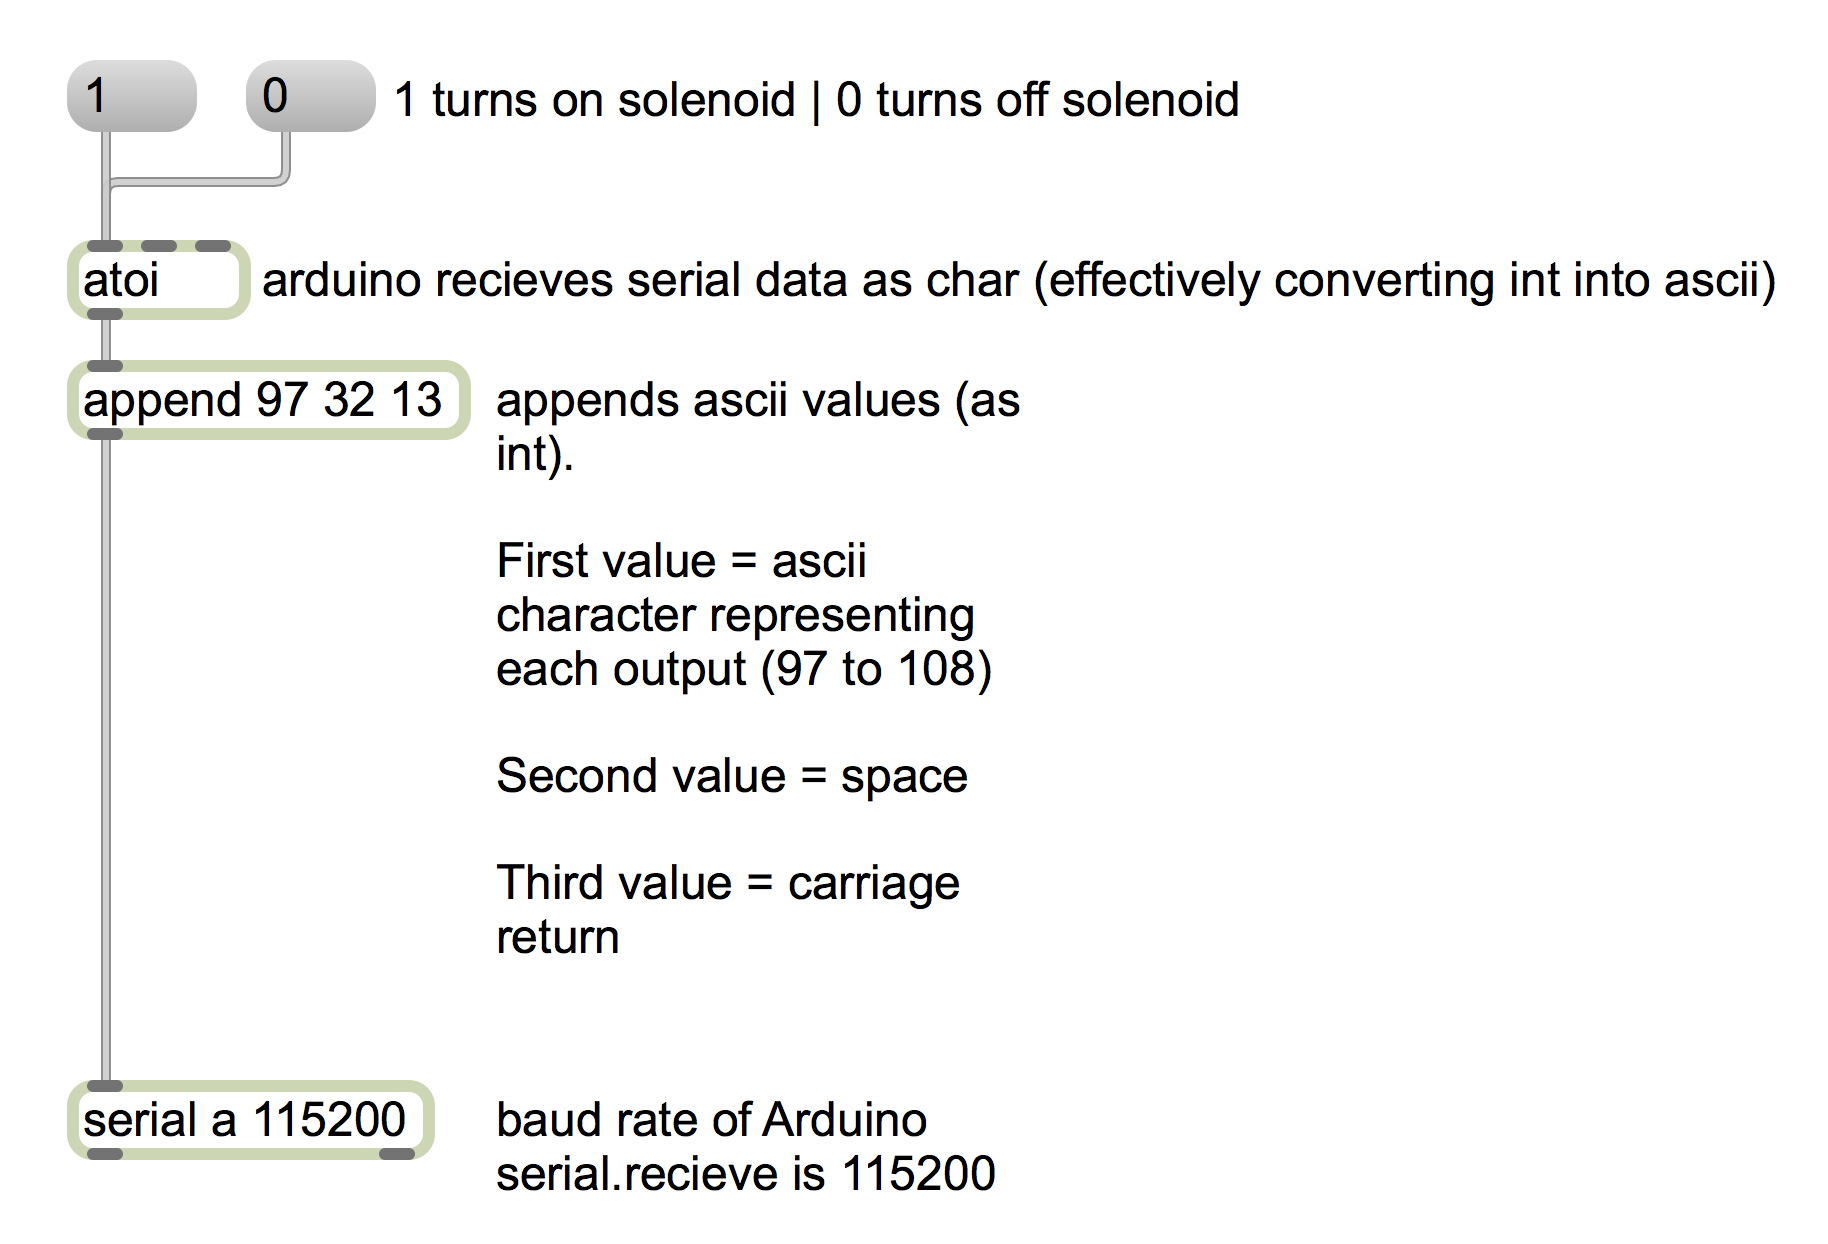
\includegraphics{../images/sol-makerSimpleExample.png}

\section{Dynamics:}
Originally \emph{pulse width modulation} (PWM) was used for all supported pins with the belief that control of the output voltage would be useful for the dynamic capability of the solenoids. This was unfortunate because the Arduino Uno only supports 6 pins for PWM. It became apparent, however, that PWM was unnecessary since the velocity of the solenoids can be effectively controlled with the hold-time--the length of time that current is pushed through a solenoid. Thus, if a solenoid is given current for 10ms it will hit with less force than if current is held for 20ms. Each solenoid is likely to have idiosyncrasies and thus a method of calibration would be useful\footnote{A microphone is likely a requirement for such an operation. I.e.  A microphone would have to be placed near the device and it's sound energy output measured at various stages (5ms, 10ms, 20ms, etc). Once the sound energy hit it's maximum (maximum dB), the maximum current holding value is found. Each solenoid would have to undergo this process and it would depend greatly on the distance from the object being struck. If the solenoid was to be moved in any way, it would likely have to be re-calibrated. Furthermore, this calibration process could be used to create a table for midi value scaling. Nonetheless, this can all be done by ear, although not with optimum effect} but a simple scaling of MIDI velocity (0 - 127) with a range of 5 - 100ms should suffice.

\section{Future Improvements:}
\begin{itemize}
\item A multiplexer could be used to increase number of solenoids. An alternative would be to use an 	Arduino Mega which supports a larger number of digital output pins. 
\item Since the shield obscures the Arduino completely a serial send/receive light on the board would be useful.
\item  With an Arduino network adapter shield the system could easily utilize Open Sound Control (OSC) making the whole system more user friendly. Otherwise a simple MIDI input port would be sufficient for greater usability.
\item To reduce the cost of manufacturing, the circuit could be redesigned to fit an Arduino Mini.
\item To prevent accidentally plugging the power supply in with the polarity reversed, the circuit could be redesigned to include a diode at the power input. 
\end{itemize}


\end{document}
